\documentclass{article}
\usepackage[magyar]{babel}
\usepackage[utf8]{inputenc}
\usepackage{t1enc}
\usepackage{graphicx}
\usepackage{geometry}
 \geometry{
 a4paper,
 total={210mm,297mm},
 left=20mm,
 right=20mm,
 top=20mm,
 bottom=20mm,
 }
\usepackage{amsmath}
\usepackage{amssymb}
\frenchspacing
\usepackage{fancyhdr}
\pagestyle{fancy}
\lhead{Urbán János tanár úr feladatsorai}
\chead{C05/07/1. csoport}
\rhead{Függvények}
\lfoot{}
\cfoot{\thepage}
\rfoot{}

\usepackage{pgf,tikz}
\usepackage{enumitem}
\usepackage{multicol}
\usepackage{calc}
\newenvironment{abc}{\begin{enumerate}[label=\textit{\alph*})]}{\end{enumerate}}
\newenvironment{abc2}{\begin{enumerate}[label=\textit{\alph*})]\begin{multicols}{2}}{\end{multicols}\end{enumerate}}
\newenvironment{abc3}{\begin{enumerate}[label=\textit{\alph*})]\begin{multicols}{3}}{\end{multicols}\end{enumerate}}
\newenvironment{abc4}{\begin{enumerate}[label=\textit{\alph*})]\begin{multicols}{4}}{\end{multicols}\end{enumerate}}
\newenvironment{abcn}[1]{\begin{enumerate}[label=\textit{\alph*})]\begin{multicols}{#1}}{\end{multicols}\end{enumerate}}
\setlist[enumerate,1]{listparindent=\labelwidth+\labelsep}

\newcommand{\degre}{\ensuremath{^\circ}}
\newcommand{\tg}{\mathop{\mathrm{tg}}\nolimits}
\newcommand{\ctg}{\mathop{\mathrm{ctg}}\nolimits}
\newcommand{\arc}{\mathop{\mathrm{arc}}\nolimits}
\renewcommand{\arcsin}{\arc\sin}
\renewcommand{\arccos}{\arc\cos}
\newcommand{\arctg}{\arc\tg}
\newcommand{\arcctg}{\arc\ctg}

\parskip 8pt
%\title{c05-1-07-03fv}
\begin{document}

\section*{Függvények}

\subsection*{2006.03.08.}
Ábrázoljuk a következő függvényeket:
\begin{enumerate}
\item $x \mapsto |x+3|$
\item $x \mapsto |x|-4$
\item $x \mapsto |x|+|x-2|$
\item $x \mapsto |x|-|x-1|$
\item $x \mapsto |x+2|-|x-2|$
\item $x \mapsto |2x-1|$
\item $x \mapsto |2x|-|x|$
\item $x \mapsto |2x+1|+|2x-1|$
\item $x \mapsto ||x|-4|$
\item $x \mapsto ||x-2|-4|$
\end{enumerate}

\subsection*{2006.03.14.}
\begin{enumerate}
\item $x \mapsto |||x|-4|-2|$
\item $x \mapsto||x|-3|+1$
\item $x \mapsto ||x|-|x-1||$
\item $x \mapsto |x|+|x-3|+|x+1|$
\item $x \mapsto ||x|+|x-3|-4|$
\item $x \mapsto ||x+2|-|x-2||$
\item $x \mapsto |x+1|+|x|+|x-1|+|x-2|$
\item $x \mapsto |3x-2|-|2x-3|$
\end{enumerate}

\subsection*{2006.03.23.}
\begin{enumerate}
\item Ábrázoljuk a következő derékszögű koordináta-rendszerben a következő függvényeket:
\begin{abc}
\item $x \mapsto 2x+1$;
\item $x \mapsto ||x|-|x-4||$;
\item $x \mapsto |x+3|+|x|+|x-2|$;
\item $x \mapsto ||x|+|x-3|-6|$;
\item $x \mapsto |3x-4|+|2x+3|$;
\end{abc}
\item Oldjuk meg a következő egyenleteket:
\begin{abc}
\item $|x-3|=2$;
\item $||x|-4|=2$.
\end{abc}
\end{enumerate}

\subsection*{2006.03.28.}
Ábrázoljuk a következő függvényeket:
\begin{enumerate}
\item $x \mapsto 3x-2$;
\item $x \mapsto -\frac{1}{2}x+1$;
\item $x \mapsto -2x+3$;
\item $x \mapsto |x-4|$;
\item $x \mapsto |x|-4$;
\item $x \mapsto ||x|-4|$;
\item $x \mapsto |2x-3|+|4x+2|$;
\item $x \mapsto ||2x-3|-|4x+2||$;
\item $x \mapsto |x|+|x-3|-|x+1|$;
\item $x \mapsto ||x|-|x-4||$;
\end{enumerate}

\subsection*{2006.03.30.}
Ábrázoljuk a következő függvényeket:
\begin{enumerate}
\item $x \mapsto 2|x|-|x-3|$;
\item $x \mapsto |x|+|x-3|+|x+1|$;
\item $x \mapsto |x+2|+|x|+|x+2|+|x-4|$;
\item $x \mapsto |x+3|+|x+1|+|x|+|x-2|+|x-4|$;
\item $x \mapsto ||x|-2|$;
\item $x \mapsto |||x|-2|-1|$;
\item $x \mapsto 2-|x-1|$;
\item $(*)$ $ x \mapsto |x|+|x-7|+|x-6|+|x-4|+|x-8|$;
\item $x \mapsto |x+1|+|x|+|x-1|+|x-3|+|x-7|$.
\end{enumerate}

\subsection*{2006.04.05.}
\begin{enumerate}
\item Ábrázoljuk a következő függvényeket:
\begin{abc}
\item $x \mapsto -2x+1$;
\item $x \mapsto ||x|-3|$;
\item $x \mapsto |||x|-4|-2|$;
\item $x \mapsto 3-|x-2|$;
\item $x \mapsto 2|x|-|2x-1|$;
\item $x \mapsto ||x|-3|+2$.
\end{abc}
\item Öt gyufásdobozban az ábrán látható számú gyufaszál van.
Szomszédos dobozokba való átrakással érjük el, hogy minden dobozban ugyanannyi gyufaszál legyen.
\begin{center}
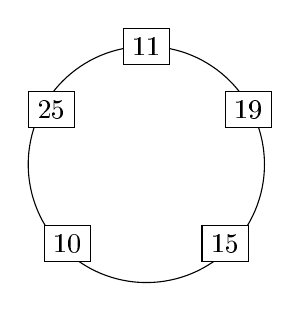
\begin{tikzpicture}[x=1.0cm,y=1.0cm, fill=white]
\draw(2,2) circle (1.5cm);
\draw (2,3.5) node[fill=white,draw] {11};
\draw (3.3,2.7) node[fill=white,draw] {19};
\draw (0.8,2.7) node[fill=white,draw] {25};
\draw (1,1) node[fill=white,draw] {10};
\draw (3,1) node[fill=white,draw] {15};
\end{tikzpicture}
\end{center}

\noindent 
 A cél a minimális számú gyufaszál átrakása. Hogyan lehet elérni?

\end{enumerate}

\subsection*{2006.04.12.}
\begin{enumerate}
\item $[x]$ jelöli azt a legnagyobb egész számot, ami nem nagyobb $x$-nél.\\ Például: 
$[2,1]=2$\quad $[-0,2]=-1$ \quad $[3]=3$\quad$0,2]=1$\quad
$[-1,3]=-2$\\
Ábrázoljuk az $x \mapsto [x]$ függvényt!
\item 
\begin{abc}
\item $x \mapsto [x]-1$;
\item $x \mapsto [x-1]$;
\item $x \mapsto 2[x]$;
\item $x \mapsto [2x]$;
\item $x \mapsto [-x]$;
\item $x \mapsto -[x]$.
\end{abc}
\end{enumerate}

\subsection*{2006.04.19.}
Ábrázoljuk a következő függvényeket:
\begin{enumerate}
\item $x \mapsto |[x]|$;
\item $x \mapsto [|x|]$;
\item $x \mapsto [x-1]$;
\item $x \mapsto [x]-1$;
\item $x \mapsto [-x]$;
\item $x \mapsto -[x]$;
\item $x \mapsto x-[x]$;
\item $x \mapsto [2x-1]$;
\item $x \mapsto 3[x]+1$;
\item $x \mapsto [x]+[-x]$.
\end{enumerate}

\subsection*{2006.04.25.}
Ábrázoljuk a következő függvényeket:
\begin{enumerate}
\item $x \mapsto x^2-1$;
\item $x \mapsto (x-1)^2$;
\item $x \mapsto -x^2$;
\item $x \mapsto -(x-1)^2$;
\item $x \mapsto [x]^2$;
\item $x \mapsto [x^2]$;
\item $x \mapsto x|x|$;
\item $x \mapsto x[x]$;
\item $x \mapsto x^2-4x+5$;
\item $x \mapsto x^2-6x+7$;
\end{enumerate}

\subsection*{2006.04.26.}
Ábrázoljuk a következő függvényeket:
\begin{enumerate}
\item $x \mapsto x^2-2x$;
\item $x \mapsto x^2-2|x|$;
\item $x \mapsto |x^2-2x|$;
\item $x \mapsto |x^2-2|x||$;
\item $x \mapsto |x^-1|$;
\item $x \mapsto x^2-4x$;
\item $x \mapsto x^2-4|x|$;
\item $x \mapsto 4|x|-x^2$;
\item $x \mapsto 4x^2-4|x|$;
\item Hol vannak a síkon azok a $P(x;y)$ pontok amelyekre teljesül, hogy $|x|+|y|\le5$?
\end{enumerate}

\subsection*{2006.04.27.}
\begin{enumerate}
\item Hol vannak a síkon azok a $P(x;y)$ koordinátájú pontok, amelyekre teljesül:
\begin{abc}
\item $|x+y|\le2$;
\item $|x-y|\le2$;
\item $y\le2x+1$ és $y\ge2x-2$.
\end{abc}
\item Ábrázoljuk a következő függvényeket:
\begin{abc}
\item $x \mapsto 2x^2$;
\item $x \mapsto 2(x-1)^2+1$;
\item $x \mapsto 2x^2+4x$;
\item $x \mapsto 2x^2+4|x|$;
\item $x \mapsto -2x^2+4|x|$.
\end{abc}
\end{enumerate}

\subsection*{2006.05.02.}
\begin{enumerate}
\item Hol vannak a síkon azok a $P(x;y)$ pontok, amelyekre teljesül:
\begin{abc}
\item $x^2-4\le y \le-x^2+4$;
\item $-x^2\le y \le x^2$;
\item $2x^2-4|x|\le y \le -2x^2+4|x|$.
\end{abc}
\item Oldjuk meg a következő egyenlőtlenségeket:
\begin{abc}
\item $x^2-4x \le 0$;
\item $x^2-4|x| \le 0$;
\item $4|x|-2x^2 \ge 0$;
\item $6|x|-x^2 \ge 0$.
\end{abc}
\end{enumerate}

\subsection*{2006.05.03.}
\begin{enumerate}
\item Ábrázoljuk a következő függvényeket:
\begin{abc}
\item $x \mapsto \frac{1}{x-1}, x\neq1$;
\item $x \mapsto \frac{1}{x+2}, x\neq-2$;
\item $x \mapsto \frac{x-3}{x-2}, x\neq2$;
\item $x \mapsto \frac{1}{|x|}, x\neq0$;
\item $x \mapsto \left|\frac{x-2}{x-1}\right|, x\neq1$;
\item $(*)$ $ x \mapsto \left[\frac{1}{x}\right], x\neq0$;
\item $x \mapsto \frac{1}{[x]}, x\ge 1, x<0$.
\end{abc}
\end{enumerate}

\subsection*{2006.05.16.}
\begin{enumerate}
\item Ábrázoljuk a következő függvényeket:
\begin{abc}
\item $x \mapsto |x^2-4|x|+3|$;
\item $x \mapsto \left|\frac{|x|-2}{|x|-1}\right|, |x|\neq1$;
\item $x \mapsto \left|\frac{x^2-6|x|+9}{|x|-3}\right|, |x|\neq3$;
\item $x \mapsto \left|\frac{|x|-3}{|x|-2}\right|, |x|\neq2$.
\end{abc}
Oldjuk meg függvények segítségével a következő egyenlőtlenségeket:
\begin{abc}
\item $x \mapsto -|x|+3\le y \le |x|-3$;
\item $x \mapsto x^2-4 \le y \le -x^2+4$;
\item $(*)$ $x \mapsto x^2-4x \le y \le 2x+5$.
\end{abc}
\end{enumerate}

\subsection*{2006.05.17.}
Ábrázoljuk a következő függvényeket:
\begin{enumerate}
\item $x \mapsto [-2x+3]$;
\item $x \mapsto |x^2-4|x||$;
\item $x \mapsto \left|\frac{|x|-1}{|x|-2}\right|, |x|\neq2$;
\item $x \mapsto \left[\frac{1}{x-1}\right], x\neq1$.
\end{enumerate}
Oldjuk meg a következő egyenlőtlenségeket:
\begin{enumerate}
\item $x^2-2x-3 \le 0$;
\item $1-\frac{1}{x-1}>0$;
\item $|x|-2 \le y \le 4-x$?
\end{enumerate}


\end{document}